\documentclass[../../../main]{subfiles}
\begin{document}

The purpose of this section is to discuss some of the challenges and benefits that is related to the use of an FPGA in this project.
\todo{refrace a bit}
The FPGA connects the  microcontroller all the components on the pan-tilt system in order to be able to control the system. It collects the data from encoders and homeing sensors, and it creates and updates the PWM signal to each of the H-Bridges.
\\
One of the main differences between an FPGA and a microcontroller is that on an FPGA everything is implemented in hardware. This also means that all of the processes running, is running in parallel. When implementing the different components this needs to be taken into consideration.
\subsection{System overview}%
\label{sub:system_overview}
\begin{figure}[H] 
    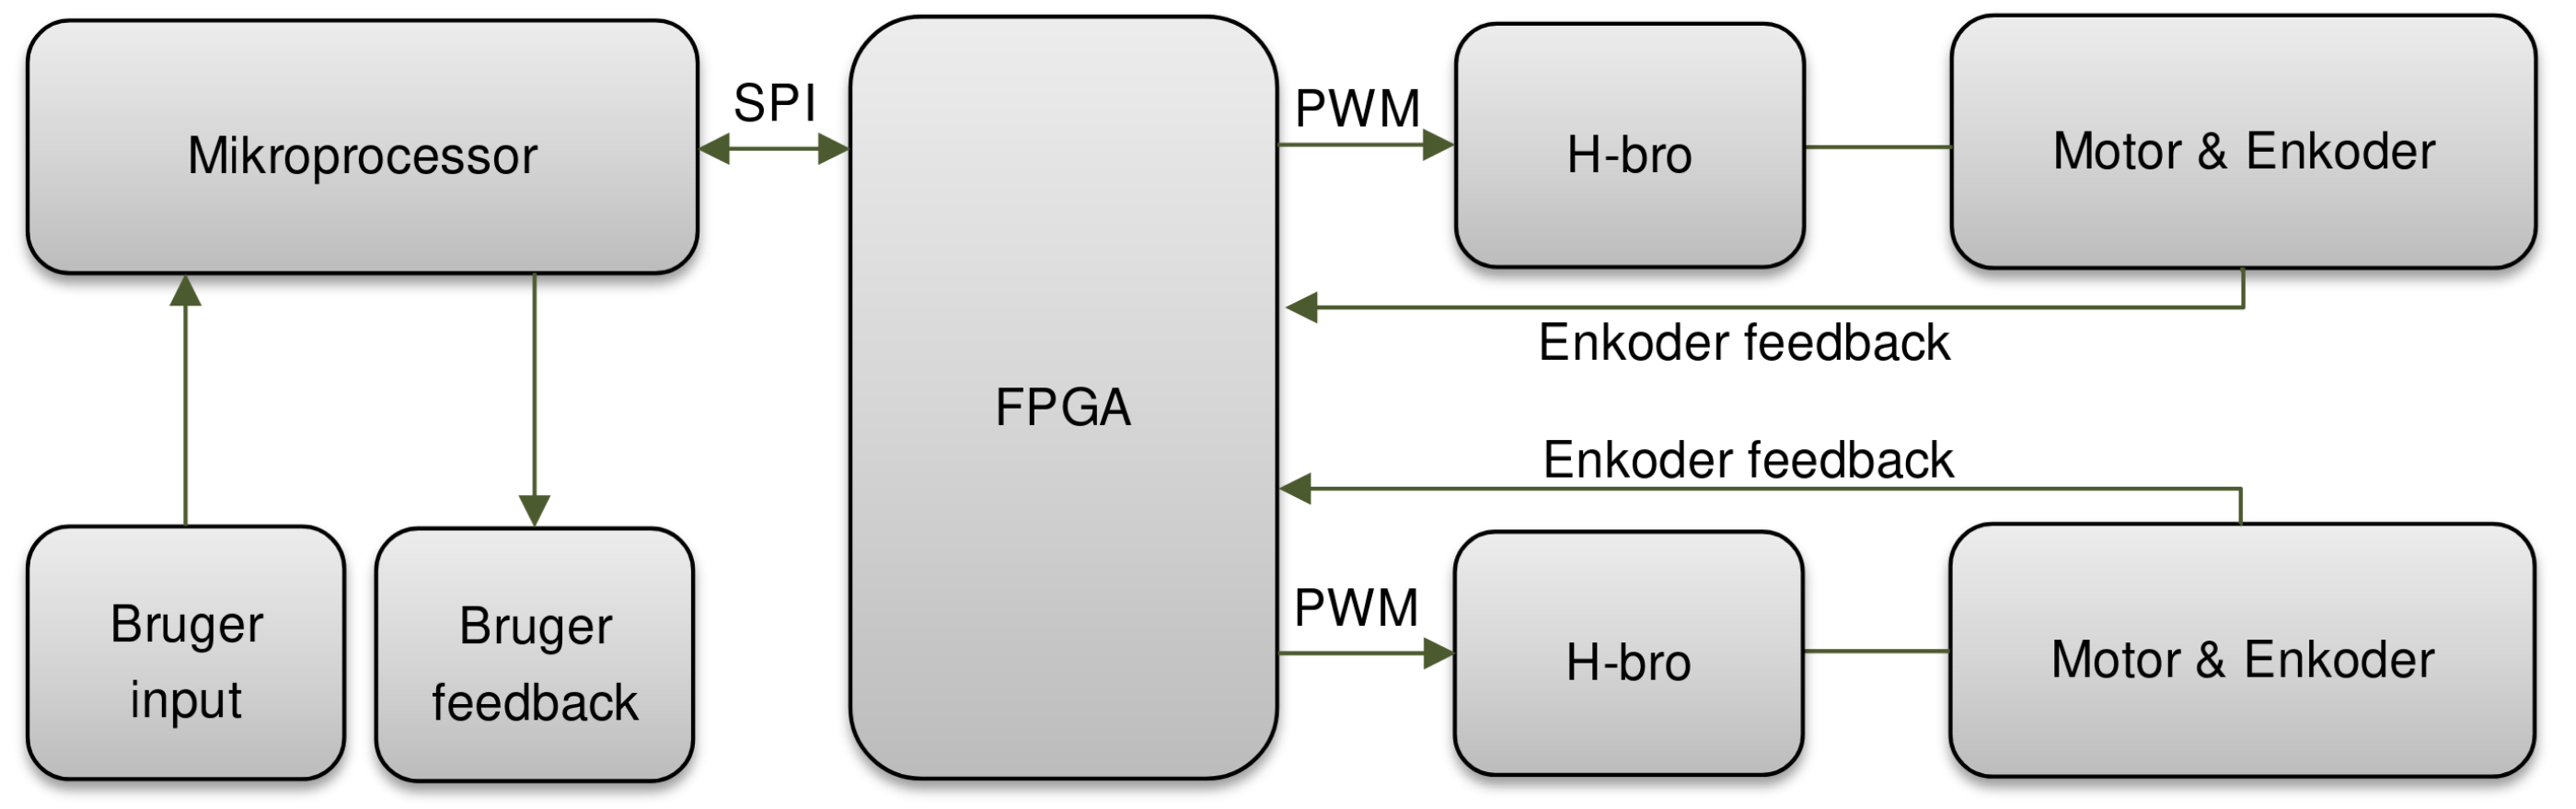
\includegraphics[width = \textwidth]{\main /afsnit/system_implementation/FPGA/images/system_overwiev.png}
    \caption {System overview}
    \label{fig:system_overview_FPGA}
\end{figure}
\todo{FIX make English / maby anoter diagram for the fpga internaly (like RTL Design) }
The system consist of different modules, implemented in VHDL. 
To store the data that needs to be exchanged between the FPGA and the Tiva microcontroller, different registers is created with the necessary size. Se table xx. \todo{create table overview of registers}
\\
The connection between the modules can be seen in figure xx. \todo{create figure}
\subsection{PWM}
The PWM module creates a PWM signal for both motors. It takes a 9 bit vector as input for each motor, and output the signals necessary for the H-Bridges to work. 
It takes the 100Mhz system clock from the FPGA as a input, and then the module contains a clock divider that creates the necessary clock frequency, for the desired PWM frequency. 
MSB in the 9 bit input vector determine witch way the motor should turn. 
The module is design so that it is possible to just define the system clock frequency and the desired PWM frequency, and the correct divider is calculated when the code is synthesized.
This is done so that it is easy to change the PWM frequency for testing.
\subsection{Protocol}
The protocol module uses a SPI module created by \todo{ref.} for communicating with the Tiva microcontroller.
The role of the protocol module is to decode the data received over SPI, and prepare data for transmission, in regards to the previously determined protocol.
%Write something about the parallel thing with the FPGA and updating of registers.

\subsection{Quadrature decoder}

\subsection{Speed measurement}
Notes to myself:\\
FPGA components:
\begin{itemize}
    \item PWM
    \item Protocol
        \begin{itemize}
            \item SPI
        \end{itemize} 
    \item Quad decoder
        \begin{itemize}
            \item Debounce
        \end{itemize}
    \item Speed mesh
\end{itemize}

\todo{describ compontens overall function, and how they communicate internaly}


\end{document}
